\documentclass[letterpaper,11pt,twoside]{article}
\usepackage[utf8]{inputenc}
\usepackage{amsmath,amsfonts,amssymb,amsthm,latexsym}
\usepackage[spanish,es-noshorthands]{babel}
\usepackage[T1]{fontenc}
\usepackage{lmodern}
\usepackage{graphicx,hyperref}
\usepackage{tikz,pgf}
\usepackage{multicol}
\usepackage{fancyhdr}
\usepackage{marvosym}
\usepackage[papersize={6.5in,8.5in}, left=1cm, right=1cm, top=1.5cm, bottom=1.7cm]{geometry}
\usepackage{fancyhdr}
\pagestyle{fancy}
\fancyhead[LE]{\Email gavendanor@colarborizadorabaja.edu.co}
\fancyhead[RE]{\url{https://www.autistici.org/mathgerman}}
\fancyhead[RO]{\Email gavendanor@colarborizadorabaja.edu.co}
\fancyhead[LO]{\url{https://www.autistici.org/mathgerman}}

\author{Germ\'an Avenda\~no Ram\'irez~\thanks{Lic. Mat. U.D., M.Sc. U.N.}}
\title{\begin{minipage}{.2\textwidth}

\includegraphics[height=1.75cm]{Images/logo-colegio.png}\end{minipage}
\begin{minipage}{.55\textwidth}
\begin{center}
Taller\\
Introducción a la ecuación de 2$^{\circ}$\\
Álgebra $9^{\circ}$
\end{center}
\end{minipage}\hfill
\begin{minipage}{.2\textwidth}

\includegraphics[height=1.75cm]{Images/logo-sed.png} 
\end{minipage}}
\date{}
\thispagestyle{plain}
\begin{document}
\maketitle
Nombre: \hrulefill Curso: \underline{\hspace*{44pt}} Fecha: \underline{\hspace*{2.5cm}}
\section*{Guía}
\subsection*{Introducción}
\begin{minipage}{.35\textwidth}
\begin{center}
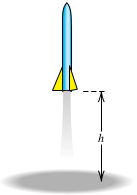
\includegraphics[scale=.8]{Images/Pantallazo-05.png}
\end{center}
\end{minipage}
\begin{minipage}{.6\textwidth}
Un cohete de juguete es lanzado verticalmente hacia arriba desde el suelo, como se ilustra en el dibujo. 
Si su rapidez inicial es de 120 pies/segundo\footnote{Un pie equivale a 12 pulgadas y una pulgada, a 2,54 cm aproximadamente} y la única fuerza que se le opone es la fuerza de gravedad, entonces la altura del cohete después de $t$ segundos está dada por la expresión
\[h=-16t^{2}+120t\]
Algunos valores de $h$ para los primeros 7 segundos de vuelo se muestran en la siguiente tabla
\end{minipage}
\begin{center}
 \begin{tabular}{|c|cccccccc|}
 \hline 
 $t$ (sec) & 0 & 1 & 2 & 3 & 4 & 5 & 6 & 7 \\ 
 \hline 
$h$ (pies) & 0 & 104 & 176 & 216 & 224 & 200 & 144 & 56 \\ 
 \hline 
 \end{tabular} 
 \end{center} 
 Podemos ver en la tabla que, al ascender el cohete, alcanza la altura de 180 pies sobre el piso en algún instante entre $t=2$ y $t=3$ segundos. Al descender, el cohete alcanza la altura de 180 pies sobre el piso en algún instante entre los 5 y 6 segundos. Para encontrar los valores exactos para los cuales $h=180$ pies, debemos solucionar la ecuación
 \[180=-16t^{2}+120t \qquad \text{ ó}\]  \[16t^{2}-120t+180=0\]
 Como se indica en el siguiente cuadro, una ecuación de esta clase se llama \emph{ecuación cuadrática en $t$}. Antes de aprender a resolver estas ecuaciones, debemos resolver el problema planteado y encontrar los instantes para los cuales el cohete se encuentra a una altura de 180 pies sobre el suelo.
 \begin{center}
 \begin{tabular}{|p{3.75cm}|p{5.5cm}|p{3cm}l|}
 \hline 
 Terminología & Definición & Ejemplos \\ 
 \hline 
Ecuación cuadrática en $x$ & Una ecuación que puede ser escrita de la forma $ax^{2}+bx+c=0$, donde $a\neq 0$ & $4x^{2}=8-11x$,\; $x(3+x)=5$, \; $4x=x^{2}$ \\ 
 \hline 
 \end{tabular} 
 \end{center}
 Para poder resolver ecuaciones de esta tipo, debemos hacer uso del siguiente teorema:
 
 \fbox{\begin{minipage}{.75\textwidth}
 Si $p$ y $q$ son expresiones algebraicas, entonces:
 \[pq=0 \qquad \text{sí y solamente sí} \qquad p=0 \quad \text{o} \quad q=0\] 
 \end{minipage}
 } 
 \subsubsection*{Ejemplo}
 Solucione la ecuación $3x^{2}=10-x$
 \paragraph*{Solución:} Para usar el método de factorización, es necesario que solamente aparezca 0 en un lado de la ecuación. Luego procedemos así:
 \begin{align*}
 3x^{2}&=10-x & \mbox{ecuación dada}\\
 3x^{2}+x-10&=0 & \mbox{sumando } x-10 \\
 (3x-5)(x+2)&=0 & \mbox{Factorizando}\\
 3x-5=0, \quad x+2&=0 & \mbox{Teorema del factor cero}\\
 x=\frac{5}{3},   \quad x&=-2 & \mbox{Solucionando para } x
 \end{align*}
 Luego las soluciones de la ecuación dada son $\frac{5}{3}$ y $-2$
\section*{Ejercicios}
\subsection*{Revisión de conceptos}
En los puntos \ref{ej01} y \ref{ej02}, llene los espacios en blanco
\begin{enumerate}
\item \label{ej01} Una ecuación de la forma $ax^{2}+bx+c=0$, donde $a$, $b$ y $c$ son números reales y $a\neq 0$, es una \underline{\hspace{1cm}} o una ecuación polinómica de segundo grado en $x$
\item \label{ej02} La parte $b^{2}-4ac$ de la fórmula general para solucionar una ecuación cuadrática se denomina \underline{\hspace*{1cm}} y determina el tipo de solución de la ecuación cuadrática.
\item Mencione cuatro métodos para solucionar una ecuación cuadrática.
\item ¿Qué representa la ecuación $S=-16t^{2}+v_{0}t+s_{0}$? ¿Qué significan $v_{0}$ y $s_{0}$?
\end{enumerate}
\subsection*{Nivel I}
 \begin{enumerate}
 \item Indica cuales de las siguientes igualdades son ecuaciones de 2$^{\circ}$ grado
 \begin{enumerate}
 \begin{multicols}{2}
 \item $x^{2}+9=25$
 \item $3x^{2}=0$
 \item $2x^{2}-7x=x^{2}-5+7x$
 \item $(x+1)^{2}-x^{2}=x+9$
 \item $3x(x+1)=2x(x+1)$
 \item $x(x-2x)=x^{2}(x-3)-1$
 \item $\dfrac{x}{3}+\dfrac{x^{2}}{6}=x^{2}$
 \item $\dfrac{6x^{2}}{5}+x^{2}=\dfrac{11x^{2}}{5}+3$ 
 \end{multicols}
 \end{enumerate}
 \item Comprueba si los valores dados a la incógnita son soluciones de la ecuación propuesta en cada caso:
 \begin{enumerate}
 \item $3x^{2}-10x+3=0$; \qquad $x=0$, $x=\dfrac{1}{3}$
 \item $2x^{2}-3x=x+2x^{2}$; \qquad $x=0$, $x=5$
 \item $(2x+1)\left(x-\dfrac{1}{3}\right)=0$; \qquad $x=1$, $x=\dfrac{1}{3}$
 \item $4(x^{2}+9)=x^{2}+144$; \; $x=6$, $x=-6$, $x=1$
 \item $\left(x-\frac{1}{2}\right)\left(\frac{1}{2}-x\right)=0$; \qquad $x=\frac{1}{2}$, $x=-\frac{1}{2}$
 \item $x(x-2)=x^{2}+1$; \qquad $x=0$, $x=\frac{1}{2}$
 \end{enumerate}
 \item Resuelva las siguientes ecuaciones incompletas:
 \begin{enumerate}
 \begin{multicols}{4}
 \item $x^{2}-9=0$
 \item $x^{2}-1=0$
 \item $x^{2}-16=0$
 \item $-x^{2}+25=0$ 
 \end{multicols}
 \end{enumerate}
 \item Resuelve las siguientes ecuaciones incompletas:
 \begin{enumerate}
 \begin{multicols}{2}
 \item $x^{2}-x=0$
 \item $-x^{2}+9x=0$
 \item $-x^{2}-10x=0$
 \item $2x^{2}+11x=0$ 
 \end{multicols}
 \end{enumerate}
 \item Resuelva las siguientes ecuaciones incompletas
 \begin{enumerate}
 \begin{multicols}{4}
 \item $x^{2}=0$
 \item $3x^{2}=0$
 \item $-x^{2}=0$
 \item $-2x^{2}=0$ 
 \end{multicols}
 \end{enumerate}
 \item Resuelva las siguientes ecuaciones completas
 \begin{enumerate}
 \begin{multicols}{2}
 \item $x^{2}+7x+12=0$
 \item $x^{2}-7x-18=0$
 \item $x^{2}+2x-15=0$
 \item $2x^{2}+11x+5=0$ 
 \end{multicols}
 \end{enumerate}
 \item Resuelva las siguientes ecuaciones:
 \begin{enumerate}
 \begin{multicols}{2}
 \item $25x(x+1)=-4$
 \item $2x(x+3)=(3(x-1)$
 \item $(2x-3)^{2}=8x$
 \item $\dfrac{x^{2}+2}{5}-\dfrac{x^{2}+x}{2}=\dfrac{3x+1}{10}$
 \item $1-5x\left(1-\dfrac{3}{2}\right)=\dfrac{x}{2}$ 
  \item $2x(3x-4)-(1-3x)(1+x)=-2$
 \end{multicols}
 \end{enumerate}
 \item Exprese matemáticamente las siguientes afirmaciones indicando si son ciertas o falsas:
 \begin{enumerate}
 \item Si al cuadrado de ocho le añado 8 unidades, obtengo setenta y seis
 \item La mitad del cuadrado de cuarenta y dos es ochocientos cuarenta
 \item Ciento cincuenta y dos disminuido en ocho unidades, da el cuadrado de doce
 \item El doble del cuadrado de 3 es 18
 \end{enumerate}
 \item La mitad del cuadrado de un número es 242. Hállelo.
 \item La suma de un número y su cuadrado es 20. Calcúlelo.
 \item Si a un número le sumo la mitad de su cuadrado, el resultado es 3/2, ¿De qué número se trata?
 \item Si a un número le sumo su triple y le resto su cuadrado, el resultado es $-5$. Halle dicho número.
 \item Solucione el problema del cohete planteado al iniciar esta guía.
 \end{enumerate}
\end{document}
